\section{Redes Neuronales}

\subsection{Brevísima historia}
\subsection{Definición}
\subsection{Multi-layer perceptron}

Una red neuronal puede pensarse simplemente como una función $f: \mathbb{R}^m \rightarrow O$ que intenta aproximar una función $f^*$ con misma aridad. Podremos notar $ y = f(x; \Theta)$, siendo $\Theta$ los parámetros de dicha función

El perceptrón, desarrollado en 1958 por Frank Rosenblatt \cite{rosenblatt1958perceptron}, intenta ajustar

\begin{equation*}
    y = H(\Theta_1 x + \Theta_0)
\end{equation*}

donde $H$ es la función de activación, y $\Theta = (\Theta_0, \Theta_1)$ son los parámetros de la función. Este modelo es el primero cuyos pesos se encontraban mediante un algoritmo, considerando que $H$ es una función derivable. Este puede considerarse como el primer modelo de una neurona, junto al modelo de McCulloch-Pitts.

\citet{minsky1969perceptrons} demostraron que este tipo de modelos sólo pueden ajustarse a datos linealmente separables, provocando el primer ``invierno'' de las redes neuronales.

Una forma de sortear estas dificultades planteadas es ``apilar'' (stack en inglés) varias de estas funciones para poder ajustar a más tipos de funciones. En términos matemáticos, esto es tan sólo una composición de funciones, tomando ahora $f = f_3 \circ f_2 \circ f_1$, donde $f_1$ es la primer ``capa'' de nuestra función correspondiente a la entrada, $f_2$ es la capa intermedia u oculta, y $f_3$ es la capa de salida. Si bien este ejemplo consta de 3 capas, se puede generalizar a arbitrarias capas ocultas. Este modelo es el que conocemos como \textbf{Perceptrón Multicapa} o \textbf{Multi-Layer Perceptron} (MLP por sus siglas en inglés)






\subsection{Redes neuronales recurrentes}

Los problemas descriptos de NLP suelen constar de procesar una secuencia de palabras o tokens $x_1, x_2, \ldots, x_k$ de longitud variable, de manera de ajustar a una función

\begin{equation*}
    y = f([x_1, \ldots, x_k])
\end{equation*}

Una manera de ajustar una función de este tipo (usando una entrada de largo fijo) es convertir este problema a ajustar una función autorregresiva

\begin{equation*}
    y_k = f(x_k, y_{k-1})
\end{equation*}

donde tenemos una salida para cada paso $k$ de tiempo. Si $f$ es una red neuronal, llamamos a este tipo de redes neuronales \textbf{recurrentes}, ya que la salida a cada paso ($y_k$) depende de la salida del paso anterior, $y_{k-1}$\footnote{No confundir con las redes neuronales recursivas}.

Una primer aproximación a este problema es la red recurrente de Elman \cite{elman1990finding} definida por las siguientes ecuaciones

\begin{align}
h_t &= \sigma(W_h x_t + U_h h_{t-1} + b_h) \\
y_t &= \sigma(W_y h_t + b_y)
\label{eq:elman}
\end{align}

$h_t$ es normalmente llamado el \textbf{estado oculto} en las redes neuronales recurrentes. Los parámetros a ajustar son $W_h, U_h$ (matrices) y $b_h, b_y$ (escalares). Podemos ver que, a grandes rasgos, este tipo de red recurrente no es nada más que un perceptrón multicapa cuya entrada consta de $x_t$, la entrada original en el tiempo actual $t$, y el estado oculto anterior, $h_{t-1}$.

Para entrenar este tipo de redes recurrentes utilizamos back-propagation through time (BPTT), que consta en desplegar la relación recurrente y aplicar back-propagation de manera normal. \todo{explicar un poco mejor esto}

Este tipo de redes recurrentes sufren de varios problemas: entre ellos, \textbf{vanishing gradient} y \textbf{exploding gradient}. Estos problemas pueden observarse ya que el cálculo del gradiente de las ecuaciones \ref{eq:elman} usando BPTT induce la potencia a la $n$ (donde $n$ es el largo de la secuencia) de las matrices $W_h$ y $U_h$. Usando la descomposición de Jordan de estas matrices, podemos ver que sus elementos en la diagonal que sean distintos de 1, o bien tienden a infinito o a cero.

El problema de \textbf{exploding gradient} puede solucionarse mediante la técnica de \textbf{gradient clipping}\todo{citation needed}, que consta de reajustar la norma del gradiente. Sin embargo, nos queda aún el problema de \textbf{vanishing gradient}. Para ello, se han propuesto otras arquitecturas recurrentes.

\citet{hochreiter1997long} propusieron las \textbf{Long Short-Term Memory} (LSTM) como solución a estos problemas. Para solucionar los problemas mencionados, proponen una arquitectura basadas en compuertas (\textbf{gates}) que regulan los cambios en el estado oculto y en la salida. Concretamente, la arquitectura de las LSTMs está regida por las siguientes ecuaciones\footnote{Para una muy buena explicación de las redes recurrentes, sugerimos este artículo: \url{https://colah.github.io/posts/2015-08-Understanding-LSTMs/}}:


\begin{align}
    h_t &= \sigma(W_h x_t + U_h h_{t-1} + b_h) \\
    y_t &= \sigma(W_y h_t + b_y)
    \label{eq:lstm}
\end{align}



\subsection{Optimización}


\section{Técnicas de representación}

Una de las necesidades que tienen las redes neuronales para poder trabajar con textos es el de tener representaciones continuas de cada token o palabra. Las representaciones utilizadas en la época previa de los modelos lineales --bolsas de palabras/caracteres ponderadas con algún esquema similar a TF/IDF-- adolecen de varios problemas: tienen una altísima dimensionalidad; no tienen representación semántica de la similaridad de las palabras; están concentradas en una o pocas dimensiones y suelen ser discretas.

Trabajo previo ha demostrado que obtener representaciones continuas y distribuidas (de manera opuesta a discretas y concentradas)

Latent Semantic Analysis (LSA) \cite{landauer1997solution} es una de las primeras técnicas de representación continua utilizadas para esta tarea. Plantean el problema de obtener representaciones continuas como el de factorizar una matriz de co-ocurrencia entre tokens y documentos (o contextos). LDA (Latent Dirichlet Allocation) \cite{blei2003latent} es otra técnica basada en modelos gráficos entrenados mediante métodos variacionales, muy utilizada aún en la actualidad ya que genera representaciones latentes de los tópicos de los textos.

\begin{figure}
    \centering
    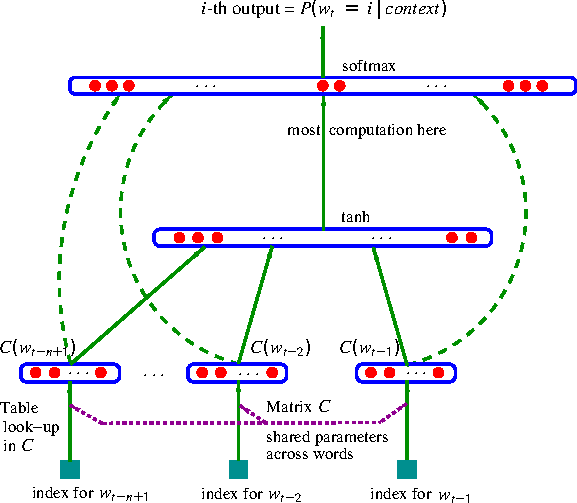
\includegraphics[width=0.65\textwidth]{img/02/bengio_neural_language_model.pdf}
    \caption{Ilustración del modelo de lenguaje neuronal de \citet{bengio2003neural}. La entrada consta de $n-1$ palabras, que primero pasan por una lookup table (o capa de embeddings), una función de activación y son colapsadas para luego ser utilizadas como entrada de una función softmax.}
    \label{fig:bengio_neural_language_model}

\end{figure}

Dentro de los métodos neuronales, uno de los más populares ha sido el de \citet{bengio2003neural} que propone una arquitectura neuronal para un modelo de lenguaje markoviano. La arquitectura de esta red está ilustrada en la figura \ref{fig:bengio_neural_language_model}. En la capa intermedia contiene una tabla de lookup de vectores de las diferentes palabras (también conocido como capa de embeddings) donde se generan las representaciones de las palabras. Trabajo posterior (con diferentes variaciones de esta misma idea) como el de \citet{collobert2011natural} ha demostrado que la utilización de este tipo de representaciones es útil para diversas tareas de NLP como POS Tagging, NER, y otras.

Uno de los problemas de los métodos vistos hasta el momento es que sufrían problemas de eficiencia, sólo pudiéndose entrenar con pocos millones de palabras y con dimensiones reducidas. La técnica \emph{word2vec} \cite{mikolov2013efficient} permite entrenar representaciones de palabras de mayor dimensión y sobre grandes cantidades de textos de manera eficiente. Los vectores de palabras guardan cierta estructura lineal y semántica, como ilustran los autores con algunos ejemplos, como el ya clásico $v(\text{rey}) - v(\text{hombre}) + v(\text{mujer}) \approx v(\text{reina})$.

Para generar los vectores de \emph{word2vec}, los autores plantean una relajación del problema de modelado de lenguaje mediante dos alternativas: Continuous Bag of Words (CBOW) y Skip-Gram. En CBOW intentamos predecir la palabra faltante dada una bolsa de palabras del contexto, y en skip-gram intentamos predecir las palabras del contexto dada la palabra central. Para ambos problemas, se generan representaciones intermedias ricas para las distintas palabras. \citet{mikolov2013efficient} extiende la idea del anterior trabajo proponiendo plantear el problema de skip-gram como uno de distinguir ruido de palabras efectivamente del contexto, haciendo mucho más eficiente el cálculo de estas representaciones. GloVe \cite{pennington2014glove} es otra técnica de representación de palabras que combina las ideas de factorización de matrices de LSA  mediante un problema de optimización distinto y generando representaciones que superan ligeramente en algunos benchmarks de tareas a los de \emph{word2vec}.

Uno de los problemas que tienen estos métodos es que cada representación se calcula sobre las distintas palabras. En español, por ejemplo, las palabras gato, gata, gatito, gatuno, todas tienen representaciones independientes en \emph{word2vec}, a pesar de tener información morfológica en común. Esto es un problema en varios escenarios: idiomas con muchas inflexiones o aglutinantes (como el turco, alemán o finés) o --lo que es de nuestro interés-- texto altamente desnormalizado como el de redes sociales. La técnica \fasttext{} \cite{bojanowski16} extiende la idea de \emph{word2vec} mediante la asignación de vectores a secuencias de 3 caracteres (subpalabras), capturando así cierta información morfológica. La representación de una palabra se obtiene mediante una combinación lineal de los vectores de las subpalabras que la componen.

\subsection{Tweet Embeddings}
\label{sec:02_tweet_embeddings}

%%
%%
%%
%%  https://docs.google.com/drawings/d/1BU3ulBiqU0NojpW6Fkb4xFlMCDigSWwfjN7z9smO6nY/edit
%%
%%

\begin{figure}[t]
    \centering
    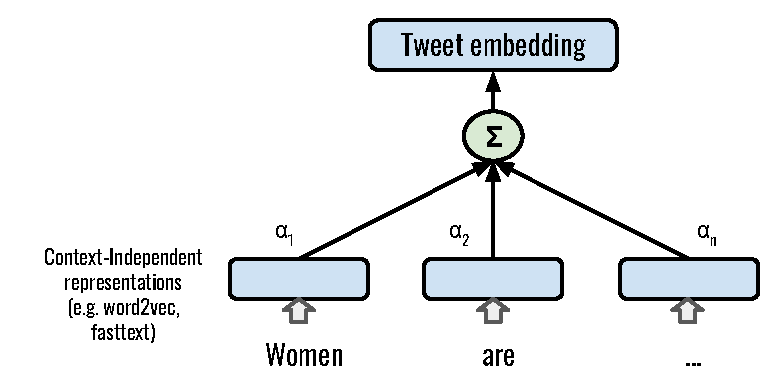
\includegraphics[width=0.80\textwidth]{img/tweet_embeddings.pdf}
    \caption{Representación contínua de un tweet mediante combinación lineal de las representaciones de cada palabra.}
    \label{fig:tweet_embeddings}
\end{figure}

Una forma relativamente simple de obtener una representación de un documento u oración (en nuestra tesis, esto será casi siempre un tweet) es realizar una combinación lineal de las representaciones obtenidas para cada palabra. Es decir, dada una oración $s = w_1 w_2 \ldots w_n$, y representaciones $\overline{w_1}, \overline{w_2}, \ldots, \overline{w_n} \in \mathbb{R}^m$, podemos obtener una representación

\begin{equation}
    \overline{s} = \sum\limits_{i=1}^{n} \alpha_i \overline{w_i}
\end{equation}

con $\alpha_1, \ldots, \alpha_n \in \mathbb{R}$ escalares (dependientes de la oración). De esta manera, obtenemos de $n$ representaciones independientes del contexto una representación para el tweet, sin tener en cuenta posibles interacciones entre los distintos componentes. La figura \ref{fig:tweet_embeddings} ilustra esta metodología simple para obtener representaciones de oraciones.

Tenemos entonces dos posibilidades para determinar la combinación lineal: la forma de obtener las representaciones, y la forma de calcular los coeficientes. Para las representaciones, podemos usar varias de las técnicas que ya vimos como word2vec, GloVe, o \fasttext{}. Para calcular los coeficientes, consideramos en nuestro trabajo dos formas. La primera, la forma canónica, calculando un promedio de las representaciones, es decir, tomando $\alpha_i = \frac{1}{n}$

Se utilizaron combinaciones lineales para calcular una representación de un solo tweet.
Seguimos dos enfoques simples: promedio simple y promedio ponderado. En el segundo caso, utilizamos un esquema que se asemeja a la frecuencia inversa suave (SIF) \cite{arora17}, inspirado TF-IDF.
Cada palabra $ w $ se pondera con $ \frac {a} {a + p (w)} $, donde $ p (w) $ es la palabra probabilidad unigrama y $ a $ es un hiperparámetro de suavizado.
Los valores altos de $ a $ significan más suavizado hacia el promedio simple.


\subsection{Modelos pre-entrenados}

\subsection{BERT}
\label{sec:02_preliminar_bert}

\subsubsection{Transfer Learning}

\subsection{Embeddings contextualizados}
\label{subsec:elmo}

Después del gran salto adelante que representó las incrustaciones de palabras independientes del contexto, llegó una nueva ola en los últimos años. En lugar de tener vectores entrenados para cada palabra, se generan representaciones dependientes del contexto para cada token dada una oración. Por ejemplo, \citet{mccann2017learned} usó un codificador LSTM profundo para traducción automática para generar vectores sensibles al contexto.

\elmo{} \cite{peters2018} es uno de estos enfoques dependientes del contexto y se basa en un modelo de lenguaje bidireccional profundo (biLM). La arquitectura del modelo de lenguaje consta de L capas de LSTM bidireccionales, además de una representación de token independiente del contexto. Por lo tanto, para cada token en una secuencia, obtenemos representaciones vectoriales de $ 2L + 1 $.
% Estas representaciones se consideran profundas ya que utilizan la salida de cada capa LSTM.
Para obtener un vector final para cada token, los autores sugieren colapsar las capas en vectores mediante una combinación lineal.

% Sea $ t_1, \ldots, t_n $ una secuencia de tokens, y sea $ h_ {k, j} $ el vector que representa la salida de la capa $ j $ cuando se consume el token $ t_k $. Entonces, el vector contextualizado para el token $ k $ es:
%
% \begin {ecuación}
% ELMo_k ^ {tarea} = \gamma ^ {tarea} \sum_ {j = 0} ^ {L} s_j h_ {k, j} \label {eq: elmo}
% \end {ecuación}

En este trabajo, usamos la implementación y los modelos entrenados previamente de \cite{che-EtAl:2018:K18-2}. El modelo español se entrenó con $L = 2 $ capas y 1024 dimensiones, y la combinación lineal se realizó utilizando un promedio simple.

% \begin{figure}
%     \centering
%     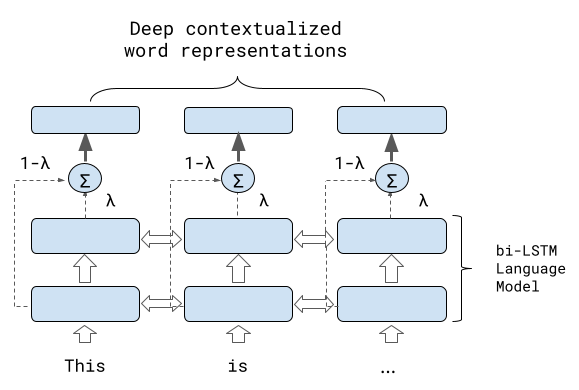
\includegraphics[width=0.65\textwidth]{img/ELMo.png}
%     \caption{Ilustración de ELMo. Las dos capas inferiores representan un modelo de lenguaje bidireccional, y la superior representa una combinación lineal convexa de las salidas de las capas recurrentes}
%     \label{fig:modelos_offenseval_hateval}
% \end{figure}
\subsection{ULM-Fit}
\subsection{BERT}

